\chapter{Experiments}\label{Experiments chapter}
In this chapter we will, through experiments, investigate what speedup one obtains by using our proposed algorithm \ref{PPC_PEN_ALG} for parallelizing optimal control problems in temporal direction. Unlike the parallel performance of gradient and objective function evaluation, the parallel performance of our overall algorithm is difficult to model. The reason for this is that it is difficult to say a-priori how many gradient and function evaluations are needed for the optimization algorithms to terminate. We are therefore unable to derive any theoretical expected speedup.
\\
\\
In section \ref{analysis sec} we explained that a good way of measuring performance of a parallel algorithm is to compare its execution time to the sequential execution time of the best sequential algorithm. We will assume that algorithm \ref{SEQ_ALG} is the best sequential algorithm for solving reducible optimal control problems. When solving optimal control problems with DE constraints, the runtime of our solution algorithm will depend on how many times we have to evaluate the objective function and its gradient, since these evaluations require either the solution of the state equation or the state and adjoint equations. We know from theory in section \ref{analysis sec} and verification in section \ref{ver S sec}, that the speedup of parallel gradient and function evaluation depends linearly on the number of processes we use. An alternative way of measuring parallel performance is therefore to compare the sum of gradient and function evaluations in the sequential and parallel algorithms. Let us give these numbers a name:
\begin{align*}
L_s &= \textit{Number of function and gradient evaluations for sequantial algorithm}\\
L_{p_N} &= \textit{Number of function and gradient evaluations for parallel algorithm using N processes}
\end{align*} 
Using these definitions we define the ideal speedup $\hat{S}$, as the speedup one would expect based on $L_s$ and $L_{p_N}$ and the speedup results we have for function and gradient evaluations:
\begin{align}
\hat S = \frac{NL_s}{L_{p_N}} \label{ideal S}
\end{align}
With $\hat S$, it is possible to say something about the performance of the parallel algorithm without having to time it, or actually run it in parallel. It will also be useful to compare the ideal speedup with the measured speedup, as a way to check if the parallel implementation is implemented efficiently.
\section{Testing the Parareal-Based Preconditioner on the Example Problem}
In this section we will test the parallel framework introduced in chapter \ref{method_chap} on our example problem (\ref{exs_J}-\ref{exs_E}). To be able to do this, we need to define a specific objective function and state equation. The problem we will look at in this section is the following:
\begin{align}
&J(y,v) = \frac{1}{2}\int_0^{T}v(t)^2dt + \frac{1}{2}(y(T)-11.5)^2,\quad T=100, \label{speed_j}\\
&\left\{
     \begin{array}{lr}
       	y'(t)=-0.097y(t) + v(t) \quad t\in(0,T)\\
       	y(0)=3.2
     \end{array}
   \right. \label{speed_e}
\end{align}
We motivate the choice of a large end time $T=100$ with the findings of section \ref{consistency_sec}. There we observed that the penalty method ran into trouble when the time steps became too small, because the error in objective function value then hit machine precision. To be able to test the problem for a large number of time steps, we therefore need a large $T$.
\\
\\
We want to test how algorithm \ref{PPC_PEN_ALG} performs when we vary the number of decompositions $N$, the penalty parameter $\mu$ and the number of fine time steps $n$. We also want to investigate how our preconditioned algorithm performs in comparison to a version of algorithm \ref{PPC_PEN_ALG} where we do not use the Parareal-based preconditioner. Most of our tests are conducted using simulated parallelism, but we also include an experiment where we test out a parallel implementation of algorithm \ref{PPC_PEN_ALG} on multiple cores.
\\
\\
In all our experiments we will use the L-BFGS algorithm\cite{nocedal1980updating} with memory length 10 to optimize the penalized objective function. We briefly explained how this algorithm works in section \ref{optiSec}. Everywhere where the Parareal-based preconditioner is used, it is constructed using a coarse propagator $\bold G_{\Delta T}$ based on the same numerical scheme as the fine solver. This means that when we use a Crank-Nicolson scheme to discretize the state and adjoint equations, $\bold G_{\Delta T}$ will also be based on Crank-Nicolson. In the cases where we have used an implicit Euler dicretization $\bold G_{\Delta T}$ is also based on implicit Euler.
\subsection{Comparing Unpreconditioned and Preconditioned Penalty Method}
In section \ref{pc sec} we introduced the Parareal preconditioner, as an approximation to the inverse Hessian. When using this preconditioner in our L-BFGS solver, we hope that the number of gradient and function evaluations needed in our algorithm will be smaller than if we do not use it. The experiment is conducted by first solving problem (\ref{speed_j}-\ref{speed_e}) without decomposing the time interval, and then solving the decomposed problem using $N=2,4,8,16,32,64,128$ decompositions. For all minimizations of the penalized objective function, we used penalty parameter $\mu=40000$. This means that we will only use one penalty iteration, as we have found this to be the most effective way to solve the decomposed example problem. To discretize the equations we have used the implicit Euler scheme with $\Delta t= \frac{T}{10^5}=10^{-3}$. For both the penalized and non-penalized problems we use L-BFGS with stop criteria:
\begin{align*}
||\nabla J||_{L^2} <10^{-5}
\end{align*}  
Since the point of this test is to compare the effectiveness of the Parareal-based preconditioner, we solve the decomposed problems with and without it. In table \ref{speed1} we have included the total number of gradient and function evaluations for the two cases as "pc L" and "non-pc L". We also measured the relative $L^2$-norm difference between the exact solution $v_e$ and all the penalized control solutions. The ideal speedup (\ref{ideal S}) is calculated for preconditioned and unpreconditioned solvers. The results of the sequential solver is presented in the first row named $N=1$, and we let $L_S=L_{p_1}$.
\\
\begin{table}[h]
\centering
\caption{Comparing unpreconditioned and preconditioned solver for test problem (\ref{speed_j}-\ref{speed_e}) using $N$ decompositions in time. Here $v_e$ denotes the exact control solution, $v_{pc}$ the preconditioned solver control solution and $v$ the unpreconditioned solver solution. $L_{p_N}$ represents total number of gradient and function evaluations used in each optimization. The ideal speedup $\hat S$ is based on this $L_{p_N}$. Notice that the preconditioned ideal speedup is significantly larger than the unpreconditioned ideal speedup for large $N$.}
\label{compare_table}
\begin{tabular}{lrrllrr}
\toprule
{}$N$ &  pc $L_{p_N}$ &  non-pc $L_{p_N}$ &       $||v_e-v_{pc}||$ &  $||v_e-v||$  &  pc $\hat{S}$ &  non-pc $\hat{S}$ \\
\midrule
1   &     13 &      13 &  0.000040 &    0.000040 &    1.00 &        1.00 \\
2   &     15 &      15 &  0.000064 &    0.000064 &    1.73 &        1.73 \\
4   &     29 &      29 &  0.000451 &    0.000472 &    1.79 &        1.79 \\
8   &     53 &      53 &  0.000483 &    0.001725 &    1.96 &        1.96 \\
16  &    109 &     175 &  0.001612 &    0.004105 &    1.90 &        1.18 \\
32  &     97 &     361 &  0.001267 &    0.008545 &    4.28 &        1.15 \\
64  &     43 &     469 &  0.001621 &    0.017026 &   19.34 &        1.77 \\
128 &     43 &     799 &  0.002712 &    0.033097 &   38.69 &        2.08 \\
\bottomrule
\end{tabular}
\end{table}
\\
There are several things of note about the results in table \ref{compare_table}. First off we see that the normed difference in control between exact and parallel solution lies in the range from $10^{-5}$ to $10^{-3}$. Another observation about the norm difference, is that for each $N$, the preconditioned and unpreconditioned solvers seems to produce roughly the same error. 
\\
\\
When we look at the total number of gradient and functional evaluations for the preconditioned and unpreconditioned solvers, we see that there are differences. While it seems to be little to no benefit to use the preconditioner for $N=2,...,8$, it becomes very important for the bigger $N$ values, where number of gradient and functional evaluations seems to explode for the unpreconditioned solver. If one accepts the above solutions as good enough, we see that we for the preconditioned solver get speedup for all decompositions, and that the ideal speedup seems to increase when we increase $N$. We do however see that the ideal speedup for each $N$ is considerably less then optimal for all $N$. Another thing that we notice when looking at the sum of gradient and function evaluations for the preconditioned solver, is that it increases steadily up to $N=16$, and then starts to decline again for higher $N$s. The reason for this is that when we increase the number of decomposed subintervals, we also make the coarse solver in the Parareal preconditioner finer. This means that the preconditioner becomes a better approximation of the Hessian, which makes the L-BFGS iteration converge faster.
\subsection{The Impact of $\mu$ on our Parareal-Based Preconditioner}
In the previous subsection we observed that the performance of our Parareal preconditioned algorithm was independent of the number decompositions $N$. In this subsection we will investigate how our method performs, when we let $N$ and $n$ be constant, but vary the penalty parameter $\mu$. The experiment will be conducted by solving problem (\ref{speed_j}-\ref{speed_e}) using a Crank-Nicolson finite difference scheme. We use $n=10^3$ and $\Delta t=0.1$. The test will be executed sequentially, and potential speedup is measured using the ideal speedup $\hat S$ defined in (\ref{ideal S}). To be able to calculate $\hat S$, we first need to solve (\ref{speed_j}-\ref{speed_e}) using the serial algorithm. We present the accuracy and total number of function and gradient evaluations $L_S$ of the serial solution in table \ref{mu1}.
\\ 
\begin{table}[h]
\centering
\caption{Number of gradient and function evaluations ($L_s$) and relative $L^2$ error ($||v_e-v||$) between exact solution $v_e$ and solution of sequential algorithm $v$.} \label{mu1}
\begin{tabular}{lrrllrr}
\toprule
{}  &  $||v_e-v||$  &  $L_S$  \\
\midrule
serial result  &     3.88e-05 &   23    \\
\bottomrule
\end{tabular}
\end{table}
\\
We then test our method on problem (\ref{speed_j}-\ref{speed_e}) for $N=16$ and $N=64$ decompositions of the time interval. The penalty parameter will vary between $10$ and $10^{10}$. We again want to see how the preconditioned solver performs in comparison with the unpreconditioned solver, and we therefore solve our example problem using both solvers. We compare the solutions $v_{pc}$ and $v$ we get using these solvers with exact solution $v_e$. We measure the performance of the solvers by counting the total number of function and gradient evaluations $L_{p_N}$ done for each solve, and compare this number with $L_S$ from table \ref{mu1}. Using $L_{p_N}$ and $L_S$, we can calculate the ideal speedup $\hat S$. The results of the above detailed experiment is presented in table \ref{mu2} and \ref{mu3}.
\\
\begin{table}
\centering
\caption{Results from solving the decomposed problem (\ref{speed_j}-\ref{speed_e}) with $N=16$. Both a preconditioned and unpreconditioned version of our method were used. The penalized objective function is minimized for increasing penalty parameters $\mu$. The columns show total function and gradient evaluations ($L_{p_{16}}$), ideal speedup $\hat S$ and relative $L^2$ error ($||v_e-v_{pc}||$). These three values are presented for both the preconditioned and unpreconditioned solver. The preconditioned parallel solver obtains an error roughly the same as the sequential solver when $\mu\geq 1000$. It also achieves a modest ideal speedup between 2 and 3, when $\mu< 10^8$. For $\mu\geq10^8$ we no longer observe a speedup greater than one for our preconditioned algorithm.}
\label{mu2}
\begin{tabular}{lrrrrrr}
\toprule
{} $\mu$&    pc $L_{p_{16}}$ & non-pc $L_{p_{16}}$  &  pc $\hat S$ & non-pc $\hat S$ &  $||v_e-v_{pc}||$ &      $||v_e-v||$\\
\midrule
1e+1     &  173 &  211 &  2.12&  1.74 &  6.8e-3 &  6.8e-3 \\
1e+2   &   99 &  357 &  3.71 &  1.03 &  6.5e-4 &   6.5e-4\\
1e+3  &  153 &  885 &  2.40 &  0.41 &  3.1e-5 &  1.1e-4 \\
1e+4 &  123 &  433&  2.99 &  0.84 &  3.2e-5 &  7.8e-5 \\
1e+5 &  155 &  379 &  2.37 &  0.97 &  3.9e-5 &  9.2e-5 \\
1e+08 &  410 &  3007 &  0.89 &  0.12 &  3.9e-5 &  4.3-2 \\
1e+10 &  388 &  3007 &  0.94 &  0.12 &  3.9e-5 &  4.8-2 \\
\bottomrule
\end{tabular}
\\
\end{table}
\begin{table}[h!]
\centering
\caption{Same as table \ref{mu2}, but now with $N=64$. We observe better ideal speedup than in table \ref{mu2} for the preconditioned solver, and the error is still roughly the same as the one measured for the sequential solver. The results achieved when solving the decomposed problem (\ref{speed_j}-\ref{speed_e}) without the Parareal-based preconditioner is worse when we use $N=64$ instead of $N=16$. We again observe significant drop in speedup when $\mu>10^5$.}
\label{mu3}
\begin{tabular}{lrrrrrr}
\toprule
{} $\mu$&    pc $L_{p_{64}}$ & non-pc $L_{p_{64}}$    &  pc $\hat S$ & non-pc $\hat S$ &  $||v_e-v_{pc}||$ &      $||v_e-v||$\\
\midrule
1e+1  &  101 &  1141 &  14.5 &  1.2 &  4.5e-2 &  4.5e-2 \\
1e+2   &  141 &  1583 &  10.4 &  0.9 &  4.7e-3 &  4.7e-3 \\
1e+3   &  169 &  1693 &   8.7 &  0.8 &  4.3-4 &  4.4e-4 \\
1e+4  &  125 &  2437 &  11.7 &  0.6 &  1.0e-5 &  1.8e-4 \\
1e+5 &  121 &  1807 &  12.1 &  0.8 &  3.4e-5 &  1.8e-4 \\
1e+08 &  439 &  3007 &   3.3 &  0.4 &  3.9e-5 &  6.7e-4 \\
1e+10 &  582 &  3007 &   2.5 &  0.4 &  3.9e-5 &  2.3e-1 \\
\bottomrule
\end{tabular}
\end{table}
\\
The results of table \ref{mu2} and \ref{mu3} again show that the preconditioned method performs better than the unpreconditioned method. This is observed in all three measures $L_{p_N}$, $\hat S$ and $||v_e-v||$ presented in the tables. For both $N=64$ and $N=16$, the total number of function and gradient evaluations $L_{p_N}$ does not differ too much when we change the penalty parameter $\mu<10^8$. This again leads to stable ideal speedup values. We also notice that the measured difference between the exact and numerical control solutions is proportional to $\frac{1}{\mu}$ until it reaches the error of the sequential solution. This is in line with what we observed in section \ref{consistency_sec} about the consistency of our method. When we do not use the preconditioner, we see that we for most of $\mu$ values fail to get a speedup larger than one, and we do not get an error of the same order as the error from the sequential algorithm. Though the speedup results of table \ref{mu3} are better than the ones shown in table \ref{mu2}, the results of both tables demonstrate that our preconditioned method can achieve speedup even for penalty parameters $\mu>10^8$. 
\\
\\
When we increase $\mu$ above $10^5$, we see for both $N=16$ and $N=64$, that $L_{p_N}$ increases. For $N=16$ we even observe speedup values less than one for the preconditioned algorithm. We can however improve the performance of our method for large $\mu$ by doing multiple penalty steps. We illustrate this with the results presented in table \ref{mu4}. Here we first solved our example problem with $\mu=10^5$ and $N=16$, and then used this solution as an initial guess to the optimization of the penalized objective function with $\mu =10^8$. We see that when we use this approach, solving the problem with $\mu=10^8$ only requires $25$ extra function and gradient evaluations. Adding these to $L_{p_{16}}=155$ from the $\mu=10^5$ solve yields a total of $180$ function and gradient evaluations, which for our example means an ideal speedup of $\hat S =2.04$. Similar results can be obtained for $N=16$.
\\
\begin{table}[h!]
\caption{Result of first solving problem (\ref{speed_j}-\ref{speed_e}) using $\mu=10^5$, for $N=16$, and then using this solution as an initial guess for the solution of the same problem using $\mu=10^8$. The two first rows present $L_{p_{16}}$, $\hat S$ and normed control error ($||v_e-v_{pc}||$) between exact solution $v_e$ and numerical solution $v_{pc}$ for each penalty iteration. The last row show the total result of both solves. Notice that going from $\mu=10^5$ to $\mu=10^8$ only requires $25$ extra function and gradient evaluations. In comparison solving problem (\ref{speed_j}-\ref{speed_e}) with $\mu=10^8$, but without a good initial guess requires $L_{p_{16}}=410$. } \label{mu4}
\begin{tabular}{lrrr}
\toprule
{} $\mu$ & $L_{p_{16}}$ & $\hat S$ & $||v_e-v_{pc}||$ \\
\midrule
1e+5 &155 &2.37 &3.85e-5\\
1e+8 &25 &14.72 &3.87e-5\\
\midrule
Overall result &180 &2.04 &3.87e-5\\
\bottomrule
\end{tabular}
\end{table}
\subsection{Speedup Results for a High Number of Decompositions} \label{Aspeed_sec}
To properly test algorithm \ref{PPC_PEN_ALG}, we have tested its use on the example problem on the Abel computer cluster. Using Abel, we are able to test our algorithm for a large number of CPUs. For all experiments the execution time of the sequential and parallel algorithms is measured by timing the solvers ten times, and choosing the lowest execution time. All our tests are done using an implicit Euler discretization. We run the test for three different problem sizes $n=6\cdot 10^5,12\cdot 10^5,24\cdot 10^5$ using an increasing number of processes $N$. Each process gets its own decomposed subinterval. The results for selected values of $N$ and $n= 24\cdot 10^5$ are found in table \ref{speed1}, while the remaining results are presented in figure \ref{speed_fig1}.
\\
\begin{table}[h]
\centering
\caption{Results gained from solving problem (\ref{speed_j}-\ref{speed_e}) for $n=24\cdot 10^5$ on $N$ processes. The first two columns shows the error in control and objective function value. $L_{p_N}$ is the total number of gradient and function evaluations, while $\hat S$ is the ideal speedup. The execution time for each $N$, and the corresponding speedup and efficiency are given in the last three columns.}
\label{speed1}
\begin{tabular}{lrlrrrrr}
\toprule
{}$N$ &   $\frac{||v-v_e||_{L^2}}{||v_e||_{L^2}}$ &     $\frac{\hat J(v)-\hat J(v_e)}{\hat{J}(v_e)}$ &   $L_{p_N}$ &     $\hat S$ &       time (s) &    speedup &        efficiency \\
\midrule
1   &  0.000002 &           -- &  19 &   1.00 &  63.37 &   1.00 &  1.000 \\
4   &  0.000018 &  2.76e-10 &  37 &   2.05 &  40.12 &   1.57 &  0.394 \\
16  &  0.000061 &  3.16e-09 &  97 &   3.13 &  28.40 &   2.23 &  0.139 \\
32  &  0.000044 &   1.65e-09 &  85 &   7.15 &  12.68 &   4.99 &  0.156 \\
48  &  0.000031 &  8.28e-10 &  73 &  12.49 &   7.05 &   8.98 &  0.187 \\
72  &  0.000021 &  3.70e-10 &  88 &  15.54 &   6.24 &  10.14 &  0.140 \\
96  &  0.000015 &  2.19e-10 &  61 &  29.90 &   3.63 &  17.45 &  0.181 \\
120 &  0.000012 &  1.72e-10 &  61 &  37.37 &   2.69 &  23.55 &  0.196 \\
\bottomrule
\end{tabular}
\end{table}
\noindent
\\
The results of table \ref{speed1} demonstrates that our parallel method can achieve actual speedup. The achieved speedup is however quite modest, since we for 120 cores only get a speedup of $23.5$. We also notice that the speedup is smaller then the ideal speedup $\hat S$. This is as expected, since $\hat S$ assumes zero parallel overhead. There are three factors that cause the parallel overhead. The first is the overhead caused by communication and hardware. It is difficult to diminish these effects, but when the problem size increase the impact of the built in overhead should decrease. The second factor is our implementation. Our code is not optimized, and this has a bigger effect on the more complicated parallel algorithm than the sequential one. The effects of a suboptimal implementation does not necessarily diminish when we increase the problem size, but we might be able to remove these effects by improving our code. The last factor that impacts the parallel overhead, is our sequential Parareal-based preconditioner. The Parareal-based preconditioner is applied to the gradient through a backward and a forward solve on a coarse mesh of size $N$. This means that the effect of the preconditioner on the parallel overhead increases when we increase the numbers of processes. If $N<<n$ these effects will however be very small. The results of table \ref{speed1} are obtained by solving a problem of size $n=24\cdot 10^5$, while the largest $N$ value is $120$, which means that N is $20000$ times smaller than $n$. It is therefore unlikely that it is the sequential Parareal-based preconditioner that is the main cause of the gap between ideal and measured speedup in table \ref{speed1}. Instead the disparity in ideal and measured speedup is probably caused by a combination of built in overhead and a suboptimal implementation.
\\
\\
Another interesting observation about table \ref{speed1}, is that the solution seems to improve when we increase $N$, which we see by looking at how the numerical control solution compares to the exact solution when we increase $N$. We compare exact and numerical solution by looking at normed difference in control and difference in function value. For $N\leq16$ these measures increase, but for $N>16$ they start to decrease again. We see the same type of pattern for $L_{p_N}$, which represents the total number of objective function and gradient evaluations done in each optimization. One interpretation of this, is that the Parareal-based preconditioner improves when the coarse decompositions become finer. The results of figure \ref{speed_fig1} paints a similar picture.
\\
\begin{figure}[!h]
\centering
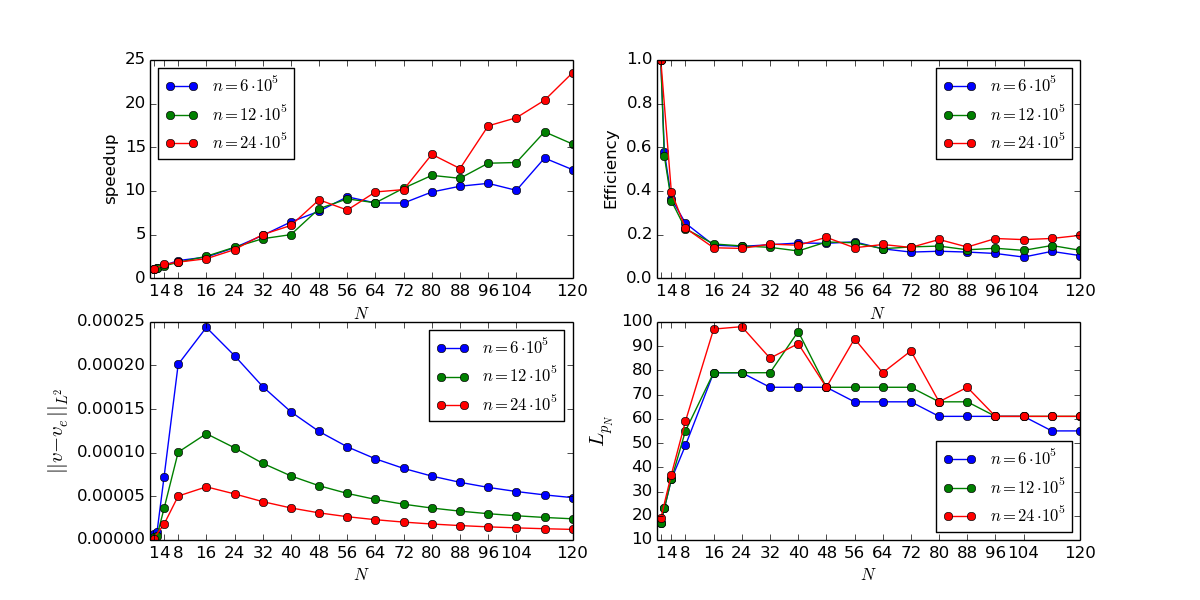
\includegraphics[scale=0.5]{fspeed_fig.png}
\centering
\caption{Speedup, efficiency, relative norm error and total number of objective function and gradient evaluations  ($L_{p_N}$) for problem (\ref{speed_j}-\ref{speed_e}) using $n=6\cdot 10^5,12\cdot 10^5,24\cdot 10^5$ time steps on $N$ cores. }
\label{speed_fig1}
\end{figure}
\\
By looking at figure \ref{speed_fig1}, we see that our algorithm preformed the best, at least in the sense of speedup, for $n=24\cdot 10^5$. We do however also observe the same type of behaviour for all values of $n$. We see that the error between exact and numerical control solution for all $n$ first increases up till around $N=16$, and then decreases and flattens out. The total number of gradient and function evaluations $L_{p_N}$ becomes larger for higher $N$'s when $N\leq 16$, but for $N>16$ $L_{p_N}$ starts to decrease slightly. We observe that for $N>16$, the effectiveness $E=\frac{S}{N}$ of our method stabilizes around $0.17$. The reason for this is that the total number of function and gradient evaluations decrease for $N>16$.  
\subsection{Tests on a Less Smooth Problem}
As we see by looking at figure \ref{smootha}, the control solution of our example problem (\ref{speed_j}-\ref{speed_e}), is very smooth. It is therefore interesting to see if our algorithm can produce good results for problems with more uneven solutions. A simple way of slightly complicating our example problem is to add a sine function to the integral in the objective function. To produce the control solution pictured in \ref{smoothb}, we alter $J$ in the following way:
\begin{align}
J(y,v) = \frac{1}{2}\int_0^{T}(v(t)-0.3\sin(t))^2dt + \frac{1}{2}(y(T)-11.5)^2, \quad T=100. \label{sinJ}
\end{align}
We will now try to minimize the altered objective function (\ref{sinJ}) coupled with the same state equation constraints as before. Since we in section \ref{Aspeed_sec} showed that our algorithm is capable of producing actual speedup, we are now only looking at ideal speedup and not wall clock speedup. In table \ref{unsmoothTab} we present results gained by applying our algorithmic framework to a Crank-Nicholson discretized minimization of the altered objective function (\ref{sinJ}) using $\Delta t = 10^{-2}$. For all decomposition sizes, the problem was solved using one penalty iteration. In an attempt to produce good results, we let the penalty parameter $\mu$ and tolerance $\tau$ vary between $10^4-10^5$ and $10^{-6}-10^{-5}$.
\\
\begin{figure}[h]
\centering
\begin{subfigure}{.5\textwidth}
  \centering
  \includegraphics[width=.8\linewidth]{smooth.png}
  \caption{Minimizer of objective function (\ref{speed_j})}
  \label{smootha}
\end{subfigure}%
\begin{subfigure}{.5\textwidth}
  \centering
  \includegraphics[width=.8\linewidth]{unsmooth.png}
  \caption{Minimizer of objective function (\ref{sinJ})}
  \label{smoothb}
\end{subfigure}
\caption{Optimal control for the unaltered and altered example problem (\ref{speed_j}-\ref{speed_e}). Notice the smoothness and simplicity of figure \ref{smootha}.}
\label{smooth}
\end{figure}
\\
It is interesting to contrast the findings of table \ref{unsmoothTab} with the results from table \ref{compare_table}. We notice that the total number of gradient and function evaluations ($L_{p_N}$) is consistently higher in table \ref{unsmoothTab}, but since this is also the case for the sequential solver, we actually observe better ideal speedup in table \ref{unsmoothTab} than in table \ref{compare_table}. This might indicate that our method has a higher potential for success on more complicated problems, where the serial solver requires a higher number of function and gradient evaluations.
\\
\begin{table}[h]
\caption{Results of applying our algorithmic framework to optimization of (\ref{sinJ}) for different decomposition sizes $N$. The columns display error ($\frac{||v_e-v||}{||v||}$), total number of gradient and function evaluations ($L_{p_N}$) and ideal speedup ($\hat S$). The error is measured between the exact solution and the numerical solution for each $N$. For all $N>1$, we observe the same order of accuracy as the serial algorithm. We also notice encouraging ideal speedup results, that are in part caused by an expensive serial solve, i.e. $L_S=L_{p_1}=53$. }
\centering
\label{unsmoothTab}
\begin{tabular}{lrrr}
\toprule
{} $N$&   $\frac{||v_e-v||}{||v||}$ &  $L_{p_N}$ &     $\hat S$ \\
\midrule
1   &  0.000015 &   53 &   1.000 \\
2   &  0.000021 &   75 &   1.413 \\
8   &  0.000012 &  129 &   3.286 \\
16  &  0.000010 &  159 &   5.333 \\
32  &  0.000010 &  131 &  12.946 \\
64  &  0.000010 &  157 &  21.605 \\
128 &  0.000036 &  161 &  42.136 \\
\bottomrule
\end{tabular}
\end{table}

